\clearpage
\setcounter{page}{8}
\begin{frame}
\frametitle{Geblockte QR-Zerlegung}
\begin{itemize}
	\item Matrix A\\
	\centering
	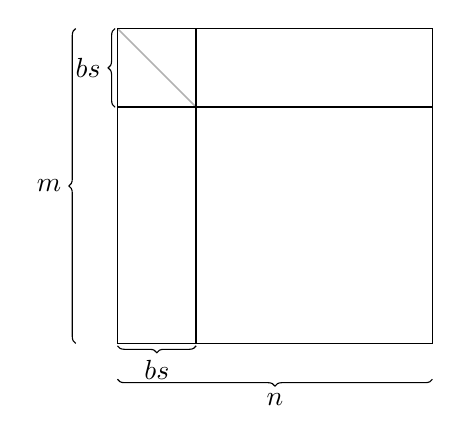
\begin{tikzpicture}
	\draw[semithick] (0,0) -- (4,0) -- (4,4) -- (0,4) -- (0,0);
	
		\draw[semithick] (1,0) -- (1,4);
		\draw[semithick] (0,3) -- (4,3);
		\draw[semithick,opacity=0.3] (0,4) -- (1,3);
		\draw[decorate, decoration={brace,mirror}, yshift=-.2ex]  (0,0) -- node[below=0.4ex] {$bs$}  (1,0);
		\draw[decorate, decoration={brace}, xshift=-.2ex]  (0,3) -- node[left=0.4ex] {$bs$}  (0,4);
	
		%\draw (0.5,3.5) node {$A_{0,0}$};
		%\draw (0.5,1.5) node {$A_{bs,0}$};
		%\draw (2.5,3.5) node {$A_{0,bs}$};
		%\draw (2.5,1.5) node {$A_{bs,bs}$};
		%\draw[decorate, decoration={brace,mirror}, yshift=-.2ex]  (0,0) -- node[below=0.4ex] {$bs$}  (1,0);
		%\draw[decorate, decoration={brace}, xshift=-.2ex]  (0,3) -- node[left=0.4ex] {$bs$}  (0,4);
		\draw[decorate, decoration={brace,mirror}, yshift=-3ex]  (0,0) -- node[below=0.4ex] {$n$}  (4,0);
		\draw[decorate, decoration={brace}, xshift=-3.5ex]  (0,0) -- node[left=0.4ex] {$m$}  (0,4);
	\end{tikzpicture}
\end{itemize}
\end{frame}

\clearpage
\setcounter{page}{8}
\begin{frame}
\frametitle{Geblockte QR-Zerlegung}
\begin{itemize}
	\item Matrix A\\
	\centering
	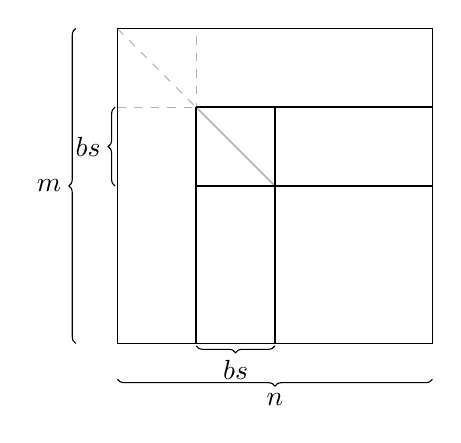
\begin{tikzpicture}
	\draw[semithick] (0,0) -- (4,0) -- (4,4) -- (0,4) -- (0,0);
	

		\draw[dashed,opacity=0.3] (1,0) -- (1,4);
		\draw[dashed,opacity=0.3] (0,3) -- (4,3);
		\draw[dashed,opacity=0.3] (0,4) -- (1,3);
		\draw[semithick] (2,0) -- (2,3);
		\draw[semithick] (1,2) -- (4,2);
		\draw[semithick] (1,0) -- (1,3);
		\draw[semithick] (1,3) -- (4,3);
		\draw[semithick,opacity=0.3] (1,3) -- (2,2);
		\draw[decorate, decoration={brace,mirror}, yshift=-.2ex]  (1,0) -- node[below=0.4ex] {$bs$}  (2,0);
		\draw[decorate, decoration={brace}, xshift=-.2ex]  (0,2) -- node[left=0.4ex] {$bs$}  (0,3);
	
	

	
	%\draw (0.5,3.5) node {$A_{0,0}$};
	%\draw (0.5,1.5) node {$A_{bs,0}$};
	%\draw (2.5,3.5) node {$A_{0,bs}$};
	%\draw (2.5,1.5) node {$A_{bs,bs}$};
	%\draw[decorate, decoration={brace,mirror}, yshift=-.2ex]  (0,0) -- node[below=0.4ex] {$bs$}  (1,0);
	%\draw[decorate, decoration={brace}, xshift=-.2ex]  (0,3) -- node[left=0.4ex] {$bs$}  (0,4);
	\draw[decorate, decoration={brace,mirror}, yshift=-3ex]  (0,0) -- node[below=0.4ex] {$n$}  (4,0);
	\draw[decorate, decoration={brace}, xshift=-3.5ex]  (0,0) -- node[left=0.4ex] {$m$}  (0,4);
	
	\end{tikzpicture}
\end{itemize}
\end{frame}

\clearpage
\setcounter{page}{8}
\begin{frame}
\frametitle{Geblockte QR-Zerlegung}
\begin{itemize}
	\item Matrix A\\
	\centering
	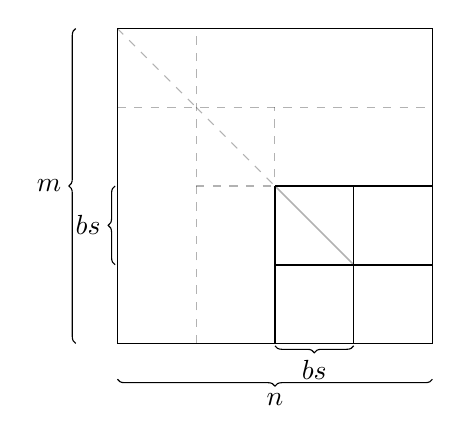
\begin{tikzpicture}
	\draw[semithick] (0,0) -- (4,0) -- (4,4) -- (0,4) -- (0,0);
	

		\draw[dashed,opacity=0.3] (1,0) -- (1,4);
		\draw[dashed,opacity=0.3] (0,3) -- (4,3);
		\draw[dashed,opacity=0.3] (0,4) -- (1,3);
		\draw[dashed,opacity=0.3] (2,0) -- (2,3);
		\draw[dashed,opacity=0.3] (1,2) -- (4,2);
		\draw[dashed,opacity=0.3] (1,3) -- (2,2);
		\draw[semithick,opacity=0.3] (2,2) -- (3,1);
		\draw[semithick] (2,1) -- (4,1);
		\draw[semithick] (3,2) -- (3,0);
		\draw[semithick] (2,2) -- (2,0);
		\draw[semithick] (2,2) -- (4,2);
		\draw[decorate, decoration={brace,mirror}, yshift=-.2ex]  (2,0) -- node[below=0.4ex] {$bs$}  (3,0);
		\draw[decorate, decoration={brace}, xshift=-.2ex]  (0,1) -- node[left=0.4ex] {$bs$}  (0,2);
	
	
	
	%\draw (0.5,3.5) node {$A_{0,0}$};
	%\draw (0.5,1.5) node {$A_{bs,0}$};
	%\draw (2.5,3.5) node {$A_{0,bs}$};
	%\draw (2.5,1.5) node {$A_{bs,bs}$};
	%\draw[decorate, decoration={brace,mirror}, yshift=-.2ex]  (0,0) -- node[below=0.4ex] {$bs$}  (1,0);
	%\draw[decorate, decoration={brace}, xshift=-.2ex]  (0,3) -- node[left=0.4ex] {$bs$}  (0,4);
	\draw[decorate, decoration={brace,mirror}, yshift=-3ex]  (0,0) -- node[below=0.4ex] {$n$}  (4,0);
	\draw[decorate, decoration={brace}, xshift=-3.5ex]  (0,0) -- node[left=0.4ex] {$m$}  (0,4);
	
	\end{tikzpicture}
\end{itemize}
\end{frame}

\clearpage
\setcounter{page}{8}
\begin{frame}
\frametitle{Geblockte QR-Zerlegung}
\begin{itemize}
	\item Matrix A\\
	\centering
	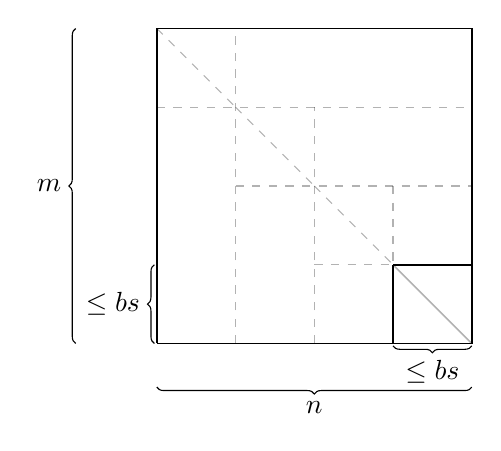
\begin{tikzpicture}
	\draw[semithick] (0,0) -- (4,0) -- (4,4) -- (0,4) -- (0,0);
	
		\draw[dashed,opacity=0.3] (1,0) -- (1,4);
		\draw[dashed,opacity=0.3] (0,3) -- (4,3);
		\draw[dashed,opacity=0.3] (0,4) -- (1,3);
		\draw[dashed,opacity=0.3] (2,0) -- (2,3);
		\draw[dashed,opacity=0.3] (1,2) -- (4,2);
		\draw[dashed,opacity=0.3] (1,3) -- (2,2);
		\draw[dashed,opacity=0.3] (2,2) -- (3,1);
		\draw[dashed,opacity=0.3] (2,1) -- (3,1);
		\draw[dashed,opacity=0.3] (3,2) -- (3,1);
		\draw[semithick] (3,1) -- (4,1);
		\draw[semithick] (3,1) -- (3,0);
		\draw[semithick,opacity=0.3] (3,1) -- (4,0);
		
	\draw[decorate, decoration={brace,mirror}, yshift=-.2ex]  (3,0) -- node[below=0.4ex] {$\le bs$}  (4,0);
	\draw[decorate, decoration={brace}, xshift=-.2ex]  (0,0) -- node[left=0.4ex] {$\le bs$}  (0,1);
	
	
	
	%\draw (0.5,3.5) node {$A_{0,0}$};
	%\draw (0.5,1.5) node {$A_{bs,0}$};
	%\draw (2.5,3.5) node {$A_{0,bs}$};
	%\draw (2.5,1.5) node {$A_{bs,bs}$};
	%\draw[decorate, decoration={brace,mirror}, yshift=-.2ex]  (0,0) -- node[below=0.4ex] {$bs$}  (1,0);
	%\draw[decorate, decoration={brace}, xshift=-.2ex]  (0,3) -- node[left=0.4ex] {$bs$}  (0,4);
	\draw[decorate, decoration={brace,mirror}, yshift=-3ex]  (0,-.1) -- node[below=0.4ex] {$n$}  (4,-.1);
	\draw[decorate, decoration={brace}, xshift=-3.5ex]  (-.5,0) -- node[left=0.4ex] {$m$}  (-.5,4);
	
	\end{tikzpicture}
\end{itemize}
\end{frame}
